\documentclass[conference,compsoc]{IEEEtran}
\IEEEoverridecommandlockouts

\ifCLASSOPTIONcompsoc
  \usepackage[nocompress]{cite}
\else
  \usepackage{cite}
\fi

\usepackage{amsmath}
\usepackage{amssymb}
\usepackage{graphicx}
\usepackage{url}
\usepackage{algorithm}
\usepackage{algorithmic}
\usepackage{hyperref}

\hyphenation{op-tical net-works semi-conduc-tor}

\begin{document}

\title{Visualizing Medical Classifier Decision Boundaries via Latent Space Traversal\thanks{Code available at \protect\url{https://github.com/theantagonist9509/capstone}.}}

\author{
 \IEEEauthorblockN{Tejas T. Singh}
    \IEEEauthorblockA{Dept. of Computer Science \& Eng.\\
    Indian Institute of Technology, Patna\\
    Email: \href{mailto:tejas_2301ai30@iitp.ac.in}{tejas\_2301ai30@iitp.ac.in}}
    \and
\IEEEauthorblockN{Rishu Kumar}
\IEEEauthorblockA{Dept. of Computer Science and Eng.\\
Indian Institute of Technology, Patna\\
Email: \href{mailto:rishu_2422cs04@iitp.ac.in}{rishu\_2422cs04@iitp.ac.in}}
\and
\IEEEauthorblockN{Shreya Yadav}
\IEEEauthorblockA{Dept. of Computer Science and Eng.\\
Indian Institute of Technology, Patna\\
Email: \href{mailto:shreya_2422cs20@iitp.ac.in}{shreya\_2422cs20@iitp.ac.in}}
\and
    \IEEEauthorblockN{Rajiv Misra}
    \IEEEauthorblockA{Dept. of Computer Science \& Eng.\\
    Indian Institute of Technology, Patna\\
    Email: \href{mailto:rajivm@iitp.ac.in}{rajivm@iitp.ac.in}}

    \and
    \IEEEauthorblockN{Supratik Mukhopadhyay}
    \IEEEauthorblockA{Dept. of Environmental Sciences\\
   Louisiana State University
Baton Rouge, LA 70803 \\
    Email: \href{mailto:mmukho1@lsu.edu}{mmukho1@lsu.edu}}
}

\maketitle

\begin{abstract}
We present a tool that helps clinicians judge whether to trust a binary skin lesion classifier. An EfficientNet-B0 autoencoder maps input images to a compact spatial latent space. We then traverse that space along two axes: a gradient axis, which moves classifier confidence toward a decision boundary, and a Principal Component Analysis (PCA) axis orthogonal to the gradient, which finds visually different images that hold confidence constant. Decoded frames along these paths reveal what can change while a prediction holds, and where it breaks. The key output is a boundary image; the nearest plausible image at which the classifier flips its label. To keep traversal images realistic, gradient steps are projected orthogonal to the reconstruction loss gradient, preventing out-of-distribution decodes. An interactive Gradio interface lets clinicians explore these paths, supported by Grad-CAM overlays and gamma-scaled difference maps. 
\end{abstract}
\begin{IEEEkeywords}
Interpretability, Latent Space, Autoencoder, Medical Classifier.
\end{IEEEkeywords}

\IEEEpeerreviewmaketitle

\section{Introduction}

Deep learning classifiers for medical imaging are often treated as black boxes. A clinician given a high-confidence prediction has little basis to decide whether to trust it. Explainability tools such as Grad-CAM \cite{gradcam} highlight which image regions drove a prediction, but they do not show how far an input sits from a decision boundary or what a boundary image looks like.
We address this gap by encoding skin lesion images into a compact latent space and moving through that space to find where the classifier changes its mind. Two traversal modes are provided. The gradient axis changes classifier confidence at each step by following $\nabla_z \, \sigma(\text{logit}(z))$. The PCA axis moves sideways; along directions orthogonal to this gradient; to find visually distinct images that the classifier rates equally. Decoding both paths shows what the model considers irrelevant to its decision, and what it considers critical.
We target binary classification of melanocytic nevus (NV) versus melanoma (MEL). This pair is clinically important, well-studied, and described by the ABCDE criteria (Asymmetry, Border, Color, Diameter, Evolution), which give non-experts a visual vocabulary for judging traversal results.
\begin{figure}[!t]
\centering
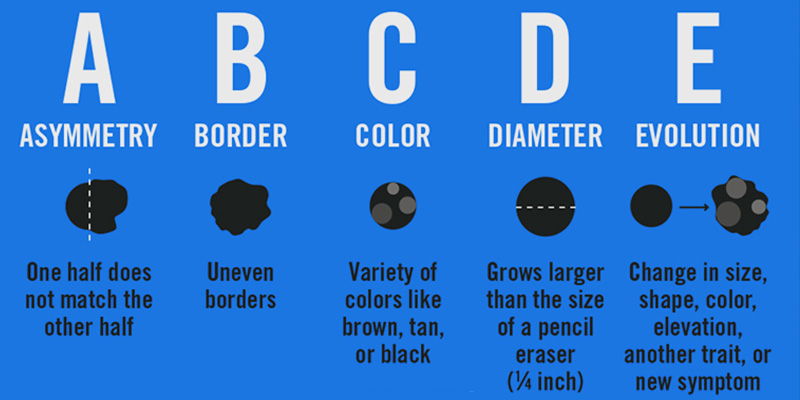
\includegraphics[width=\columnwidth]{images/abcde.jpg}
\caption{The ABCDE criteria for differentiating NV from MEL, as used by dermatologists. These visual rules make traversal results interpretable to non-experts \cite{abcde_melanoma_image}.}
\label{fig:abcde}
\end{figure}

\section{Related Work}

\subsection{Explainability in Medical Image Classifiers}

Deep learning classifiers for medical imaging routinely outperform human experts on benchmark tasks, yet their opacity has slowed clinical adoption. Saliency-based methods such as Grad-CAM \cite{gradcam} and its variants produce heatmaps highlighting which pixels drove a prediction, remaining the most widely deployed explanation tools in practice. Perturbation-based methods such as LIME \cite{lime} and SHAP \cite{shap} fit local surrogate models or compute Shapley values to attribute predictions to input features. Both families suffer from a shared limitation: they tell clinicians \emph{where} the model looked but not \emph{how far} the input sits from a different decision. Our work complements saliency maps by adding a Grad-CAM overlay to traversal frames while going further to show the nearest boundary image and the full path to it.

\subsection{Counterfactual Explanations for Image Classifiers}

Counterfactual explanations answer what smallest input change flips a model's label. Generating plausible counterfactuals is challenging because perturbations must remain on the natural image manifold. Early GAN-based approaches, including GANterfactual \cite{ganterfactual}, address this by training a conditional image-to-image translation network incorporating the target classifier. StyleGAN-based methods such as CheXplaining in Style \cite{chexstyle} manipulate disentangled latent directions in a pretrained generator to create clinically interpretable counterfactuals for chest X-rays. Diffusion autoencoders \cite{daecf} define a decision hyperplane in latent space and generate counterfactuals along its normal. For 3D imaging, Cohen et al.\ \cite{latentshift} proposed Latent Shift, updating latent codes via classifier gradients, later extended to 3D CT volumes \cite{ct3d}. Our method is closest to Latent Shift in updating latent codes via gradients, but differs by incorporating an orthogonal projection to enforce manifold constraints, a PCA traversal axis for iso-confidence exploration, and an interactive interface for skin lesion classification.

\subsection{Latent Space Traversal and Disentanglement}

A rich body of work studies moving through generative latent spaces along semantically meaningful directions. GANSpace \cite{ganspace} discovers editing directions via PCA on latent activations. InterFaceGAN \cite{interfacegan} trains a linear SVM in latent space to locate hyperplanes separating attribute classes. SeFa \cite{sefa} finds editing directions in closed form by decomposing generator layer weights. These methods target unconditional generative synthesis across global latent spaces. In contrast, we use a reconstruction autoencoder to support traversal relative to a specific external classifier. Our PCA axis is computed in the orthogonal complement of the classifier gradient on-the-fly at the current latent point.

\subsection{Skin Lesion Classification}

The HAM10000 dataset \cite{ham10000} (ISIC 2018 Task 3) contains 10,015 biopsy-confirmed dermoscopic images across seven categories and remains the standard benchmark for skin lesion classification. EfficientNet \cite{efficientnet} is the dominant backbone for this task, consistently outperforming heavier architectures on ISIC benchmarks \cite{efficientnet_skin}. Transfer learning from ImageNet is standard, using task-specific linear heads and weighted sampling to address severe class imbalance \cite{ham10000_cls}. MelanomaNet \cite{melanomanet} combines EfficientNet V2 with Grad-CAM++ attention, automated ABCDE extraction, and Monte Carlo Dropout uncertainty quantification. We build on this line of research, employing EfficientNet-B0 as both classifier backbone and autoencoder encoder, fine-tuning the classifier on reconstructions to calibrate backpropagated traversal signals.

\subsection{Variational Autoencoders and Manifold Smoothness}

Variational autoencoders \cite{vae} introduced the reparameterization trick and KL divergence regularization to encourage a smooth, connected latent manifold. Manifold smoothness is vital for traversal: rough manifolds yield non-monotonic confidence curves and visual mode jumps. The degree of KL regularization controls a trade-off between reconstruction sharpness and latent smoothness \cite{vae}. We observe this trade-off directly: our baseline autoencoder with MSE loss produces sharper reconstructions but rougher traversal, whereas the VAE yields smoother paths at the cost of softer decoded images.

\section{Methodology}

We encode an input image into a compact latent space, traverse that space
along two complementary axes to find where the classifier changes its
prediction, and decode each step back into image space for inspection.
Fig.~\ref{fig:methodology} shows the full pipeline.
Formally, let $f_{\text{enc}}$, $f_{\text{dec}}$, and $f_{\text{cls}}$
denote the encoder, decoder, and classifier respectively, and let
$z_0 = f_{\text{enc}}(x)$ be the latent code of an input image $x$.
We seek a boundary point $z^*$ such that
$f_{\text{dec}}(z^*)$ is the nearest plausible image at which
$f_{\text{cls}}$ flips its label, subject to decoded frames remaining
on the learned image manifold throughout the path.
We find $z^*$ in three stages. First, we take gradient steps in $\mathcal{Z}$
along the direction that increases classifier confidence most steeply
(Section~\ref{sec:gradient}). Second, each step is projected to remove
any component that would push the decoded image off the manifold, using
the reconstruction loss gradient as a normal to the manifold at the
current point (Section~\ref{sec:orthogonal}). Third, to explore the
neighborhood of the boundary without crossing it, we move along PCA
directions computed in the orthogonal complement of the classifier
gradient across the validation set (Section~\ref{sec:pca}). Each decoded
frame is visualized with a gamma-scaled difference overlay and a Grad-CAM
saliency map (Section~\ref{sec:visualization}).
\begin{figure}[!t]
\centering
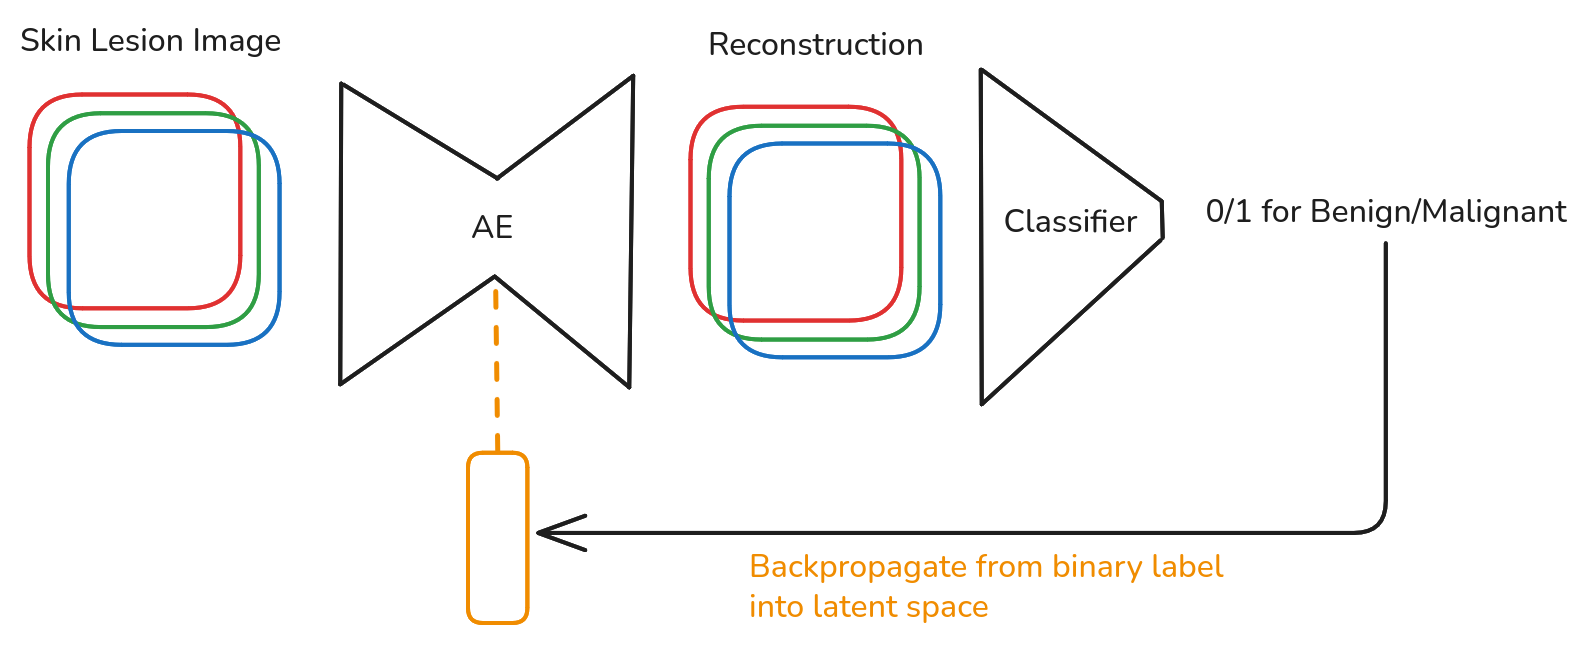
\includegraphics[width=\columnwidth]{images/flowchart.png}
\caption{Pipeline overview: an input image is encoded into $\mathcal{Z}$,
traversed via projected gradient steps until the classifier flips, and
decoded at each step for visualization. The PCA axis explores the
boundary neighborhood at constant confidence.}
\label{fig:methodology}
\end{figure}
\section{Dataset}

We initially targeted ISIC 2020 (33,000 images), but the malignant class accounted for only 1.7\% of the data, causing severe overfitting despite weighted losses. We therefore switched to HAM10000 (ISIC 2018 Task 3), which contains 10,015 biopsy-confirmed images across seven diagnostic categories, yielding a more tractable malignant rate of approximately 20\% when collapsed to binary classification. We restricted training to Melanocytic Nevus ($n = 6{,}705$) versus Melanoma ($n = 1{,}113$) to align directly with the ABCDE diagnostic criteria. To handle the 6:1 NV-to-MEL class imbalance, training uses binary cross-entropy loss with positive class reweighting and weighted random sampling to maintain balanced mini-batches. Data augmentations include random horizontal and vertical flips, rotations, and color jitter. Validation and traversal use a deterministic preprocessing pipeline: resizing to 256 pixels, center-cropping to $224 \times 224$, and normalizing with ImageNet statistics ($\mu = [0.485, 0.456, 0.406]$, $\sigma = [0.229, 0.224, 0.225]$).

\section{Model Architectures}

\noindent \textit{Classifier:}
The classifier uses an EfficientNet-B0 \cite{efficientnet} backbone pretrained on ImageNet, with the classification head replaced by a Dropout $(p{=}0.2)$ layer and a single output logit (NV vs.\ MEL; positive logit indicates MEL). Early backbone stages can optionally be frozen. Label smoothing is evaluated to prevent overly steep decision boundaries. A grayscale variant adapts the stem by summing first-layer convolution weights across input channels.

\noindent \textit{Autoencoder:}
The autoencoder shares the EfficientNet-B0 feature extractor as its encoder, mapping $224 \times 224$ RGB inputs to a spatial feature map of shape $(B, 1280, 7, 7)$. A symmetric decoder of five transposed convolution stages (with batch normalization and ReLU) progressively upsamples from $7 \times 7$ back to $224 \times 224$:
\begin{equation}
\begin{aligned}
1280 &\xrightarrow{4 \times 4,\ s2} 512 
     &\xrightarrow{4 \times 4,\ s2} 256 \\
     &\xrightarrow{4 \times 4,\ s2} 128 
     &\xrightarrow{4 \times 4,\ s2} 64 \\
     &\xrightarrow{4 \times 4,\ s2} 3
\end{aligned}
\end{equation}
The output layer has no activation, maintaining normalized image space consistency.

\noindent \textit{Variational Autoencoder:}
The VAE extends the autoencoder with a spatial variational bottleneck using $1 \times 1$ convolutions to output mean $\mu$ and log-variance $\log \sigma^2$ maps ($d = 1024$). During training, latent vectors are sampled via:
\begin{equation}
   z = \mu + \epsilon \odot \exp\!\left(\tfrac{1}{2} \log \sigma^2\right), \quad \epsilon \sim \mathcal{N}(0, I) 
\end{equation}
At inference, $z = \mu$. A Sigmoid final layer bounds output pixels to $[0, 1]$, and the objective incorporates a KL divergence term:
\begin{equation}
    \mathcal{L}_{\text{KL}} = -\tfrac{1}{2} \mathbb{E}\!\left[1 + \log \sigma^2 - \mu^2 - \exp(\log \sigma^2)\right]
\end{equation}
KL regularization improves manifold smoothness and traversal monotonicity at the cost of slight reconstruction blur.

\section{Latent Space Traversal}

\subsection{Gradient Axis}
\label{sec:gradient}

The gradient traversal optimizes the latent code $z$ to move the classifier's output toward the decision boundary. At each step, the gradient of the classifier logit with respect to $z$ is computed by decoding $z$ and backpropagating through both the decoder and the classifier:
\begin{equation}
    G = \nabla_z \; f_{\text{cls}}\!\left(f_{\text{dec}}(z)\right)
\end{equation}
The direction of travel is determined by the initial prediction: steps move \emph{along} $G$ for NV images (pushing toward MEL) and \emph{against} $G$ for MEL images (pushing toward NV). An Adam optimizer updates $z$ at each step with a default learning rate of 0.05. The gradient is recomputed at every step so it tracks the local manifold geometry, which matters because the vanilla AE latent space has no smoothness incentive between in-distribution points. Traversal stops when the predicted probability crosses a configurable threshold (default 0.75) past the decision boundary.

\subsection{Orthogonal Projection}
\label{sec:orthogonal}
Unconstrained gradient steps often push $z$ off the learned manifold, producing decoded images with synthetic colour artifacts. To address this, we project each gradient step to be orthogonal to the reconstruction loss gradient $V = \nabla_z \, \mathcal{L}_{\text{recon}}(z)$, where the reconstruction error is the MS-SSIM loss between $f_{\text{dec}}(z)$ and $f_{\text{dec}}(f_{\text{enc}}(f_{\text{dec}}(z)))$. The projection is:
\begin{equation}
 G \leftarrow G - \frac{G^\top V}{\|V\|^2} V   
\end{equation}
This removes the component of the classifier gradient that increases reconstruction error, keeping decoded images on or near the learned image manifold. The encoder pass in $V$ is detached so gradients only flow through the first decoder call, preventing interference between the two gradient computations.
\subsection{PCA Axis}
\label{sec:pca}
The PCA traversal moves sideways in latent space: it finds directions that are orthogonal to the classifier gradient and span maximum variance across the validation set's embeddings. Given a batch of encoded validation images $X \in \mathbb{R}^{B \times d}$ and the classifier gradient $G$ as the reference vector, the method (implemented in \texttt{get\_orthogonal\_pca\_bases}) first removes from each embedding its projection onto $G$:
\begin{equation}
    X_{\perp} = X - \frac{X G^\top}{\|G\|^2} G
\end{equation}
It then mean-centers $X_\perp$ and takes the top-$k$ right singular vectors via full SVD. These form the PCA bases in the orthogonal complement of $G$. Stepping along these bases at each iteration keeps the classifier score approximately constant while moving the image through visually distinct configurations that are well-supported by the training distribution.
\subsection{Visualization}
\label{sec:visualization}
Each traversal frame is decoded from the updated $z$ and unnormalized back to RGB using the ImageNet statistics. The visualization layout shows the full traversal strip in a top row and a four-panel comparison in a bottom row. The comparison panels show: the original reconstruction, the final reconstruction, a luminance-weighted scalar difference map (computed as $(I_{\text{final}} - I_{\text{orig}}) \cdot [0.299, 0.587, 0.114]^\top$, displayed with a diverging colormap), and a per-channel gamma-scaled overlay. The overlay computes the signed per-channel difference, compresses its magnitude with $\gamma = 0.5$ (preserving sign), normalizes each channel to $[0,1]$, and blends with the original at $\alpha = 0.6$:
\begin{equation}
    \text{overlay} = (1 - \alpha) \cdot I_{\text{orig}} + \alpha \cdot H_\gamma
\end{equation}
This makes subtle changes visible even when the orthogonal constraint keeps traversal steps small.

\section{Reconstruction Quality Refinements}
\label{sec:reconstruction-refinements}

Good traversal requires the autoencoder to reconstruct images faithfully enough that the classifier performs similarly on reconstructions as on originals. Early iterations fell short of this: a baseline autoencoder produced reconstructions too blurred for the classifier to trust, which a perceptual loss sharpened only partially, and a structural similarity loss finally closed the gap. The three subsections below trace that progression.

\subsection{Baseline Autoencoder}
The baseline AE with mean squared error (MSE) loss produced heavily blurred reconstructions. Classifier performance on these reconstructions was significantly worse than on originals, which undermines traversal because the gradient signal backpropagated through the decoder reflects a corrupted view of the image.

\begin{figure}[!t]
\centering
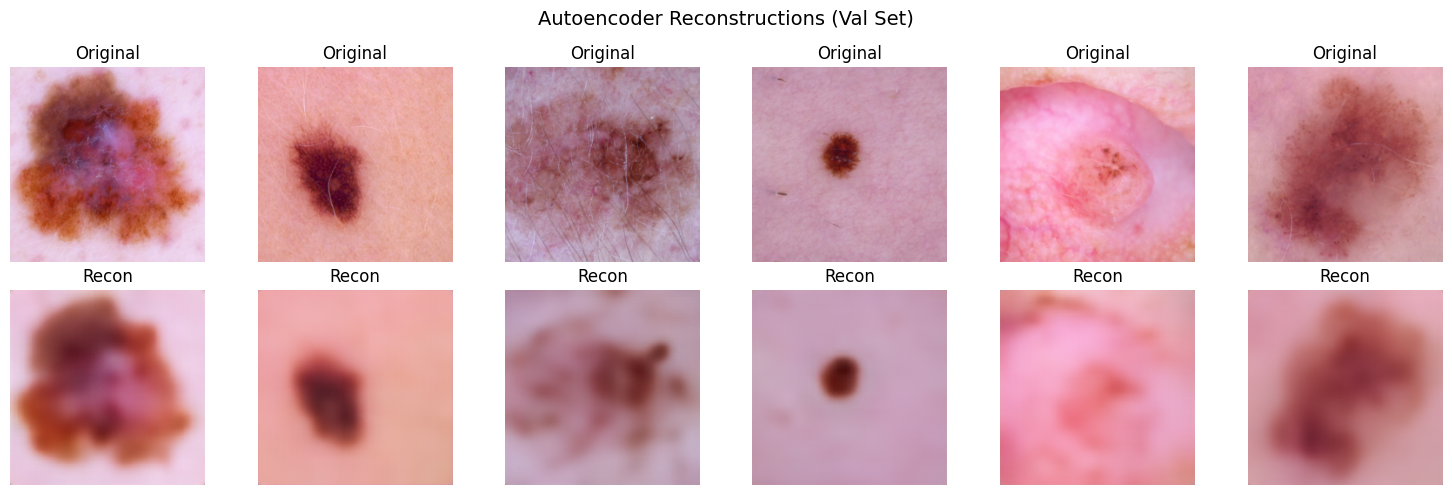
\includegraphics[width=\columnwidth]{images/ae.png}
\caption{Baseline AE reconstructions with MSE loss. The output is excessively blurry, degrading classifier performance on reconstructed images.}
\label{fig:ae}
\end{figure}

\subsection{VGG Perceptual Loss}

Replacing MSE with VGG-based perceptual loss \cite{vggloss} improved sharpness and classifier performance on reconstructions, but the results still fell short of our target. Perceptual loss matches feature distributions in VGG's intermediate layers, encouraging texture consistency rather than pixel-level accuracy.
\begin{figure}[!t]
\centering
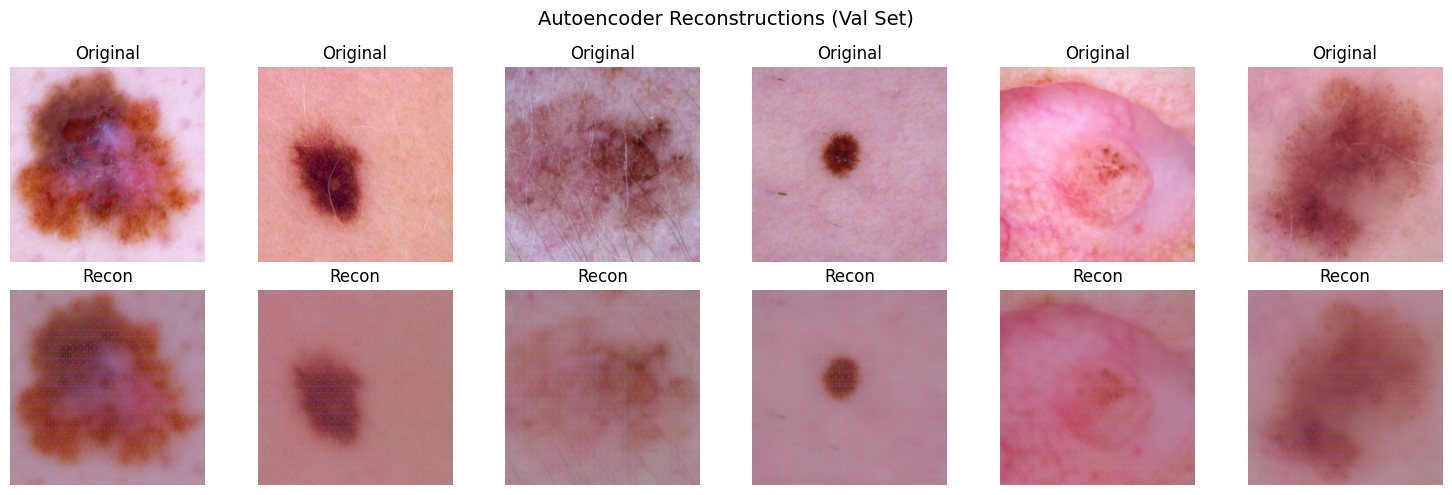
\includegraphics[width=\columnwidth]{images/ae-vgg.png}
\caption{AE reconstructions with VGG perceptual loss. Sharpness improves over baseline MSE but classifier performance on reconstructions remains below target.}
\label{fig:ae-vgg}
\end{figure}

\subsection{MS-SSIM Loss}

MS-SSIM loss \cite{msssim} outperformed VGG loss on both reconstruction sharpness and classifier performance on reconstructed images. MS-SSIM measures structural similarity across multiple scales, making it more sensitive to clinically relevant texture and edge detail. This is the loss used in our final traversal pipeline. Some gap between original and reconstructed classifier performance remains; future work may close it by combining MS-SSIM and VGG terms or adopting a GAN-style decoder.

\begin{figure}[!t]
\centering
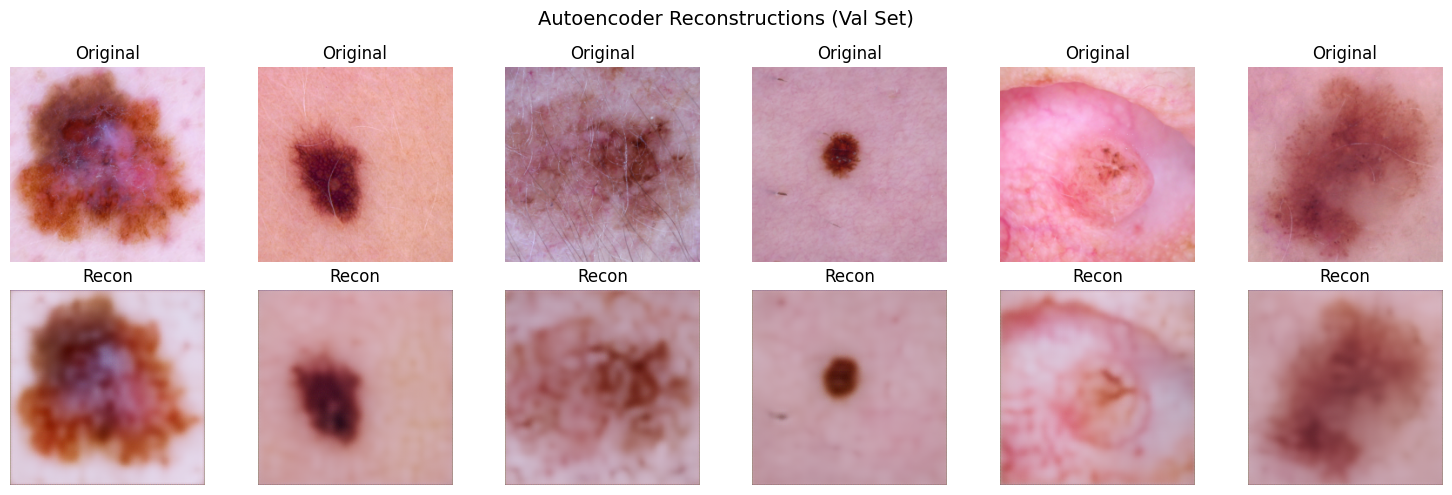
\includegraphics[width=\columnwidth]{images/ae-ms-ssim.png}
\caption{AE reconstructions with MS-SSIM loss. This yields the best reconstruction quality and classifier performance among the losses tested.}
\label{fig:ae-ms-ssim}
\end{figure}

\section{Classifier Refinements}

\subsection{EfficientNet-B2}

To test whether a larger encoder backbone would improve classification, we trained an EfficientNet-B2 classifier alongside the B0 baseline. Even with heavy regularisation (dropout $p = 0.4$), B2 validation performance was worse than B0, as shown in Fig.~\ref{fig:b0} and Fig.~\ref{fig:b2}. B0 is strictly superior across all tracked metrics. This points to a lack of data: the additional capacity of B2 cannot be used productively when the training set is this small, and the extra parameters overfit despite the added dropout. All subsequent experiments use B0.
\begin{figure}[!t]
\centering
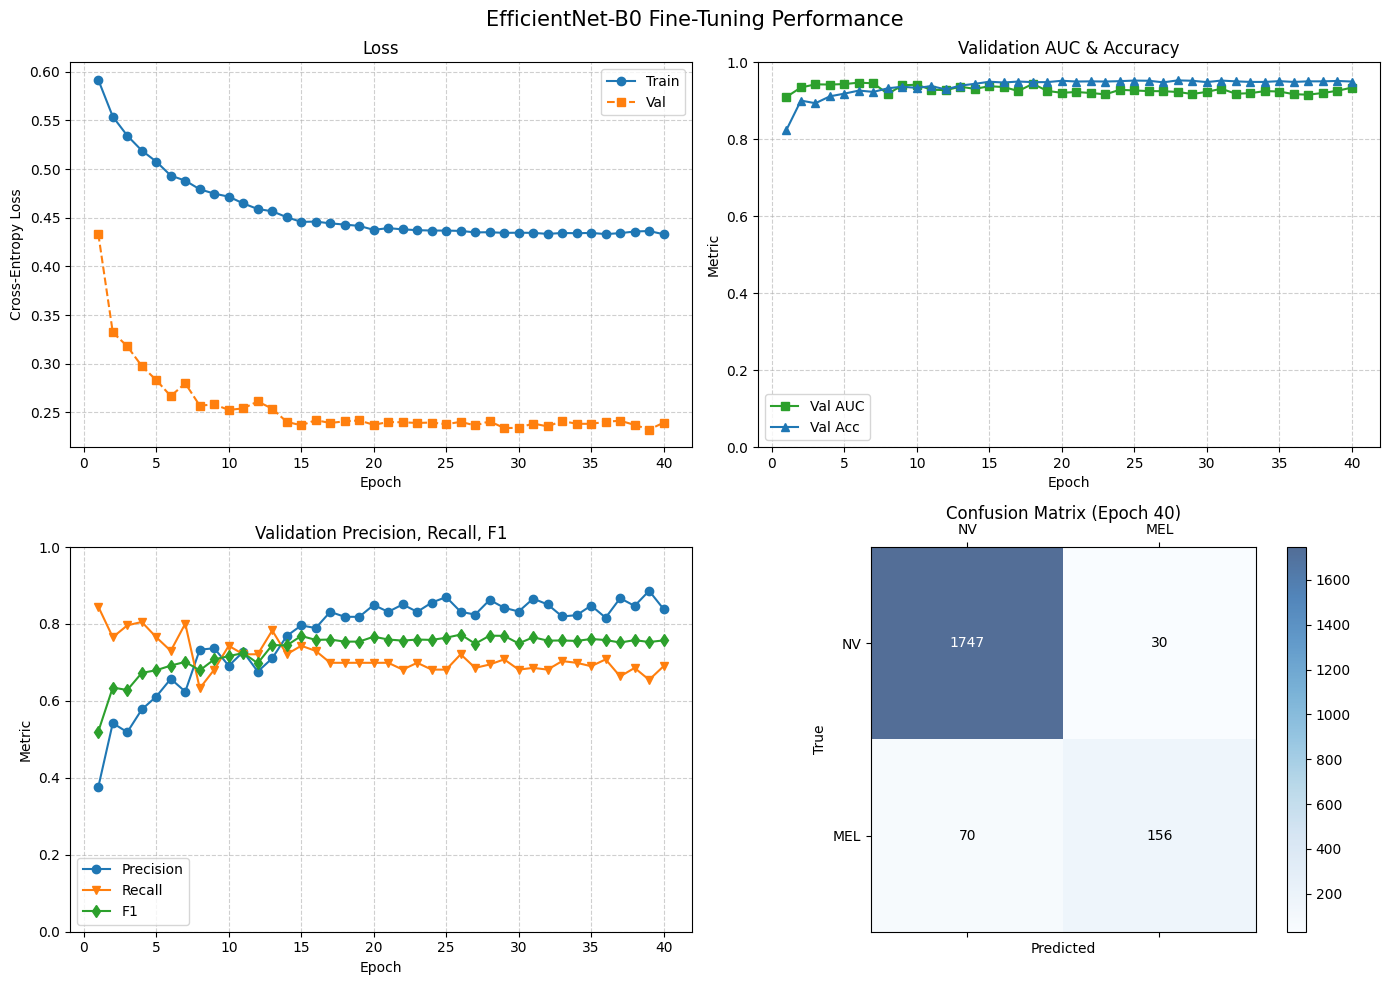
\includegraphics[width=\columnwidth]{images/b0.png}
\caption{EfficientNet-B0 validation performance. Metrics are stable and consistently higher than the B2 variant.}
\label{fig:b0}
\end{figure}

\begin{figure}[!t]
\centering
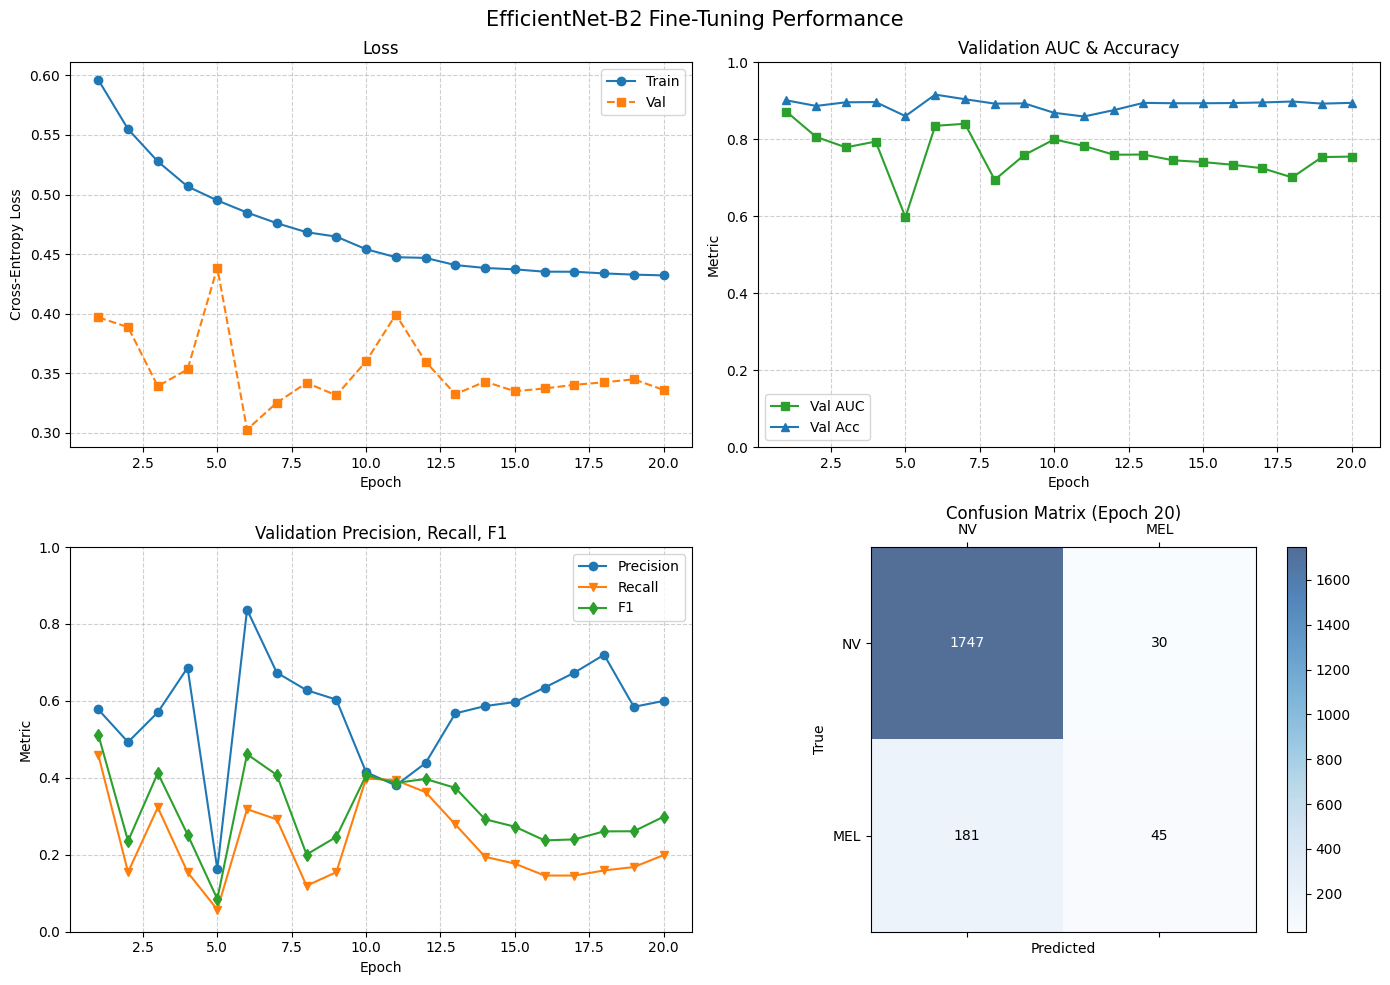
\includegraphics[width=\columnwidth]{images/b2.png}
\caption{EfficientNet-B2 validation performance with $p = 0.4$ dropout. Despite heavier regularisation, B2 underperforms B0, indicating the dataset is too small to benefit from the larger backbone.}
\label{fig:b2}
\end{figure}

\subsection{Label Smoothing}

Without label smoothing, a binary cross-entropy objective can drive logits to large positive and negative values. A steep decision boundary that passes through latent space in a near-vertical wall makes traversal steps large and imprecise; the classifier flips its label abruptly rather than smoothly. Label smoothing replaces hard $\{0, 1\}$ targets with soft targets $\{\epsilon/2,\, 1 - \epsilon/2\}$, which means the optimal logit for any class is finite. This bounds the logits and prevents the decision boundary from becoming excessively steep.
Label smoothing does not guarantee a unimodal class-probability distribution, and a bimodal distribution of predicted probabilities may persist if the data itself clusters into two well-separated groups. But by keeping logits bounded, it removes the incentive for the model to push every prediction toward near-zero or near-one confidence, which is a prerequisite for a traversable boundary. Fig.~\ref{fig:no-ls} and Fig.~\ref{fig:ls} show the effect on the predicted-probability distribution before and after label smoothing is applied.
\begin{figure}[!t]
\centering
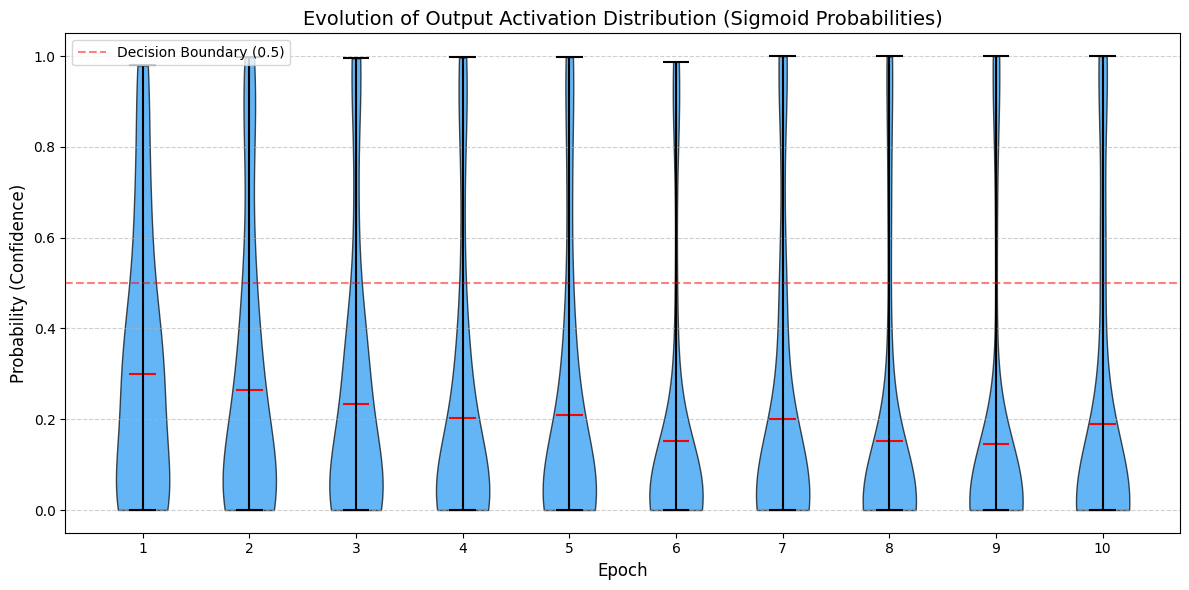
\includegraphics[width=\columnwidth]{images/no-ls.png}
\caption{Predicted class-probability distribution without label smoothing. Logits are pushed to extremes, concentrating predictions near zero and one.}
\label{fig:no-ls}
\end{figure}

\begin{figure}[!t]
\centering
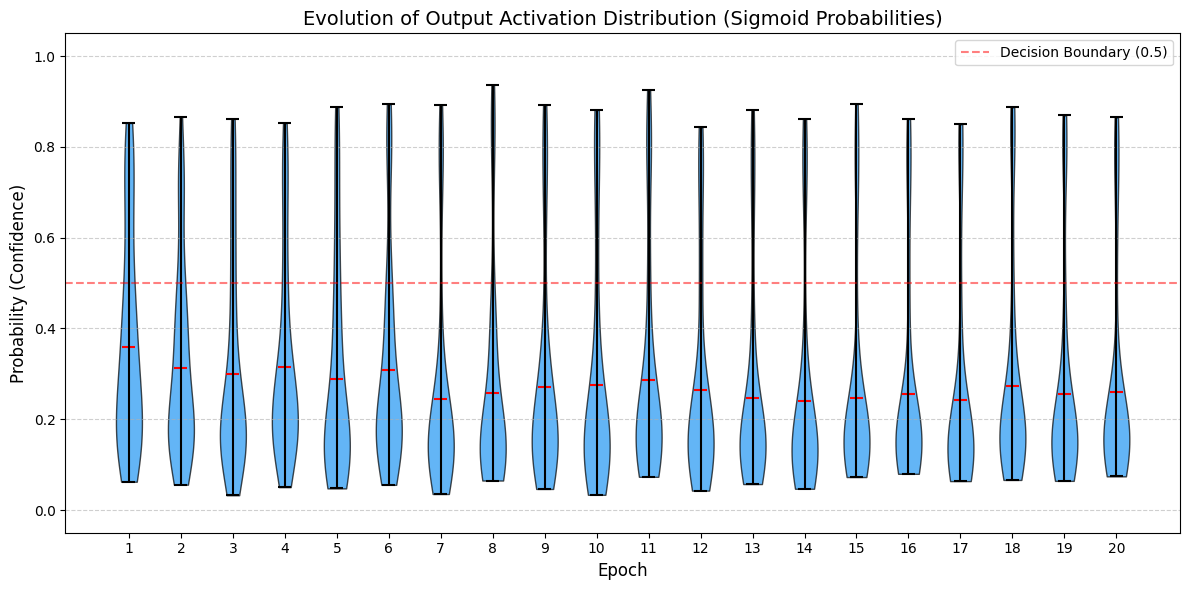
\includegraphics[width=\columnwidth]{images/ls.png}
\caption{Predicted class-probability distribution with label smoothing ($\epsilon = 0.3$) applied. Logits are bounded, spreading predictions across a wider range and producing a less steep decision boundary.}
\label{fig:ls}
\end{figure}
\subsection{Fine-Tuning on Reconstructions}

Ideally, the classifier would remain untouched: a clinician-facing tool should explain the predictions of a fixed, independently trained model rather than one adapted to suit the pipeline. In practice, a classifier trained on clean images responds poorly to AE distortions, producing gradient signals that reflect reconstruction noise rather than lesion features. Due to compute and time constraints, we fine-tuned the classifier directly on AE reconstructions to correct for this, at the cost of explaining a model that has learned to tolerate those distortions rather than the intended one. This bounds the experiment to a slightly weaker result, but provides a solid sanity check that the research direction is sound. Decoupling the classifier from the AE is a clear target for future work.
\section{Traversal Refinements}

\subsection{VAE for Manifold Smoothness}
Early AE traversals showed non-monotonic classifier confidence along the gradient direction, suggesting the latent manifold was rough. Switching to the VAE improved smoothness, as the KL regularization pulls the latent distribution toward a Gaussian prior and discourages gaps and discontinuities in the latent space.

\begin{figure}[!t]
\centering
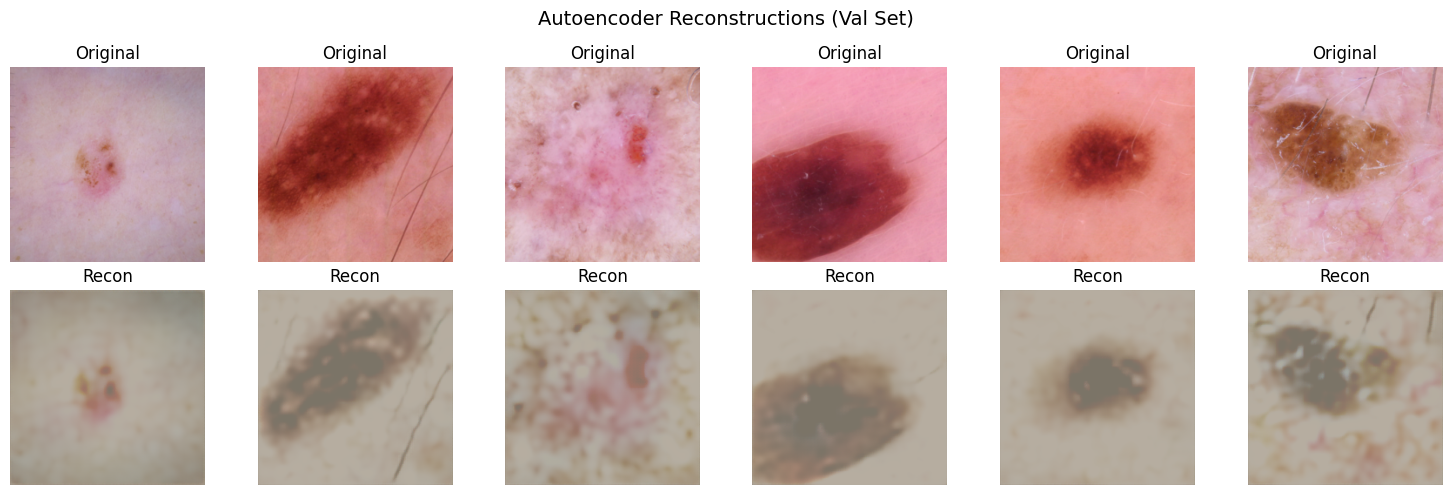
\includegraphics[width=\columnwidth]{images/vae.png}
\caption{VAE reconstructions. The smoother latent manifold reduces non-monotonic confidence during traversal at the cost of slightly softer reconstructions compared to the AE.}
\label{fig:vae}
\end{figure}

\subsection{Grayscale Training}

We tested training on grayscale images to reduce colour artifacts in traversed frames. The grayscale variants of both the classifier and AE adapted the EfficientNet-B0 stem by summing the three input channel weights into one. However, grayscale classifier performance was worse than RGB, and the approach was abandoned.

\begin{figure}[!t]
\centering
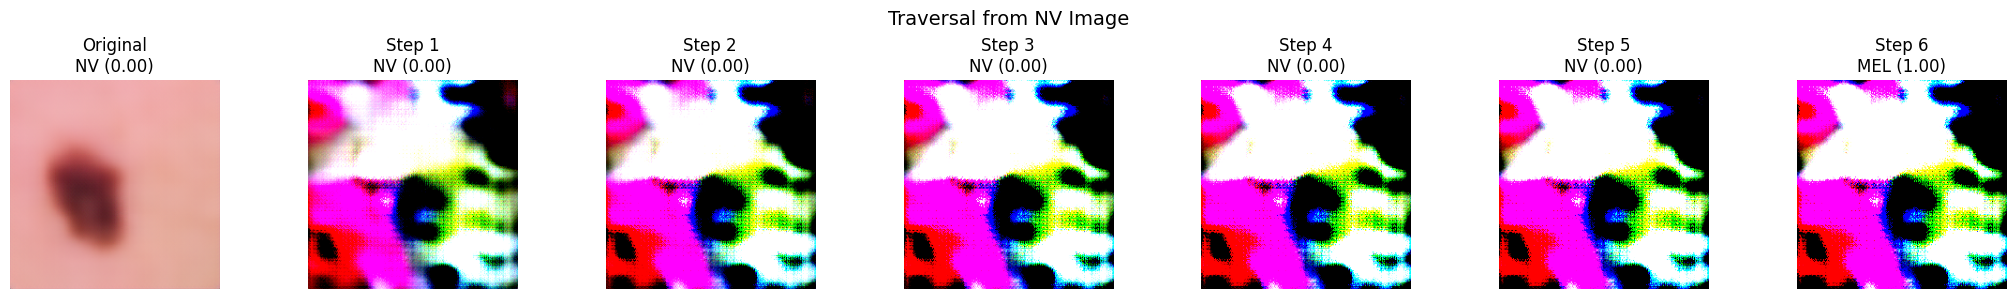
\includegraphics[width=\columnwidth]{images/artifacts.png}
\caption{Colour artifacts observed during unconstrained RGB traversal. These synthetic-looking colours indicate out-of-distribution decoded images.}
\label{fig:artifacts}
\end{figure}

\subsection{Orthogonal Traversal}

The orthogonal projection described in Section~\ref{sec:orthogonal} was the most effective fix for colour artifacts. Out-of-distribution decoded images incur a large reconstruction loss gradient; projecting away from this gradient keeps decoded images on the learned image manifold, eliminating most synthetic-looking artifacts.
\subsection{Difference Map Overlay}

Because the orthogonal constraint reduces visible changes between traversal steps, a gamma-scaled per-channel difference overlay is blended onto the original image to highlight subtle but meaningful changes. The $\gamma = 0.5$ compression amplifies small differences while the signed treatment preserves both the direction and spatial location of changes.

\subsection{Interpolation with Grad-CAM}
We added a latent-space interpolation feature that linearly mixes the latent codes of two validation-set images and decodes the resulting path. At each interpolation step, Grad-CAM \cite{gradcam} highlights which image regions drive the classifier's prediction, giving spatial attribution alongside confidence scores. This makes the latent space structure more transparent: the user can observe how classifier attention shifts smoothly as the image morphs from one example to another.

\section{Interactive GUI}

\begin{figure}[!t]
\centering
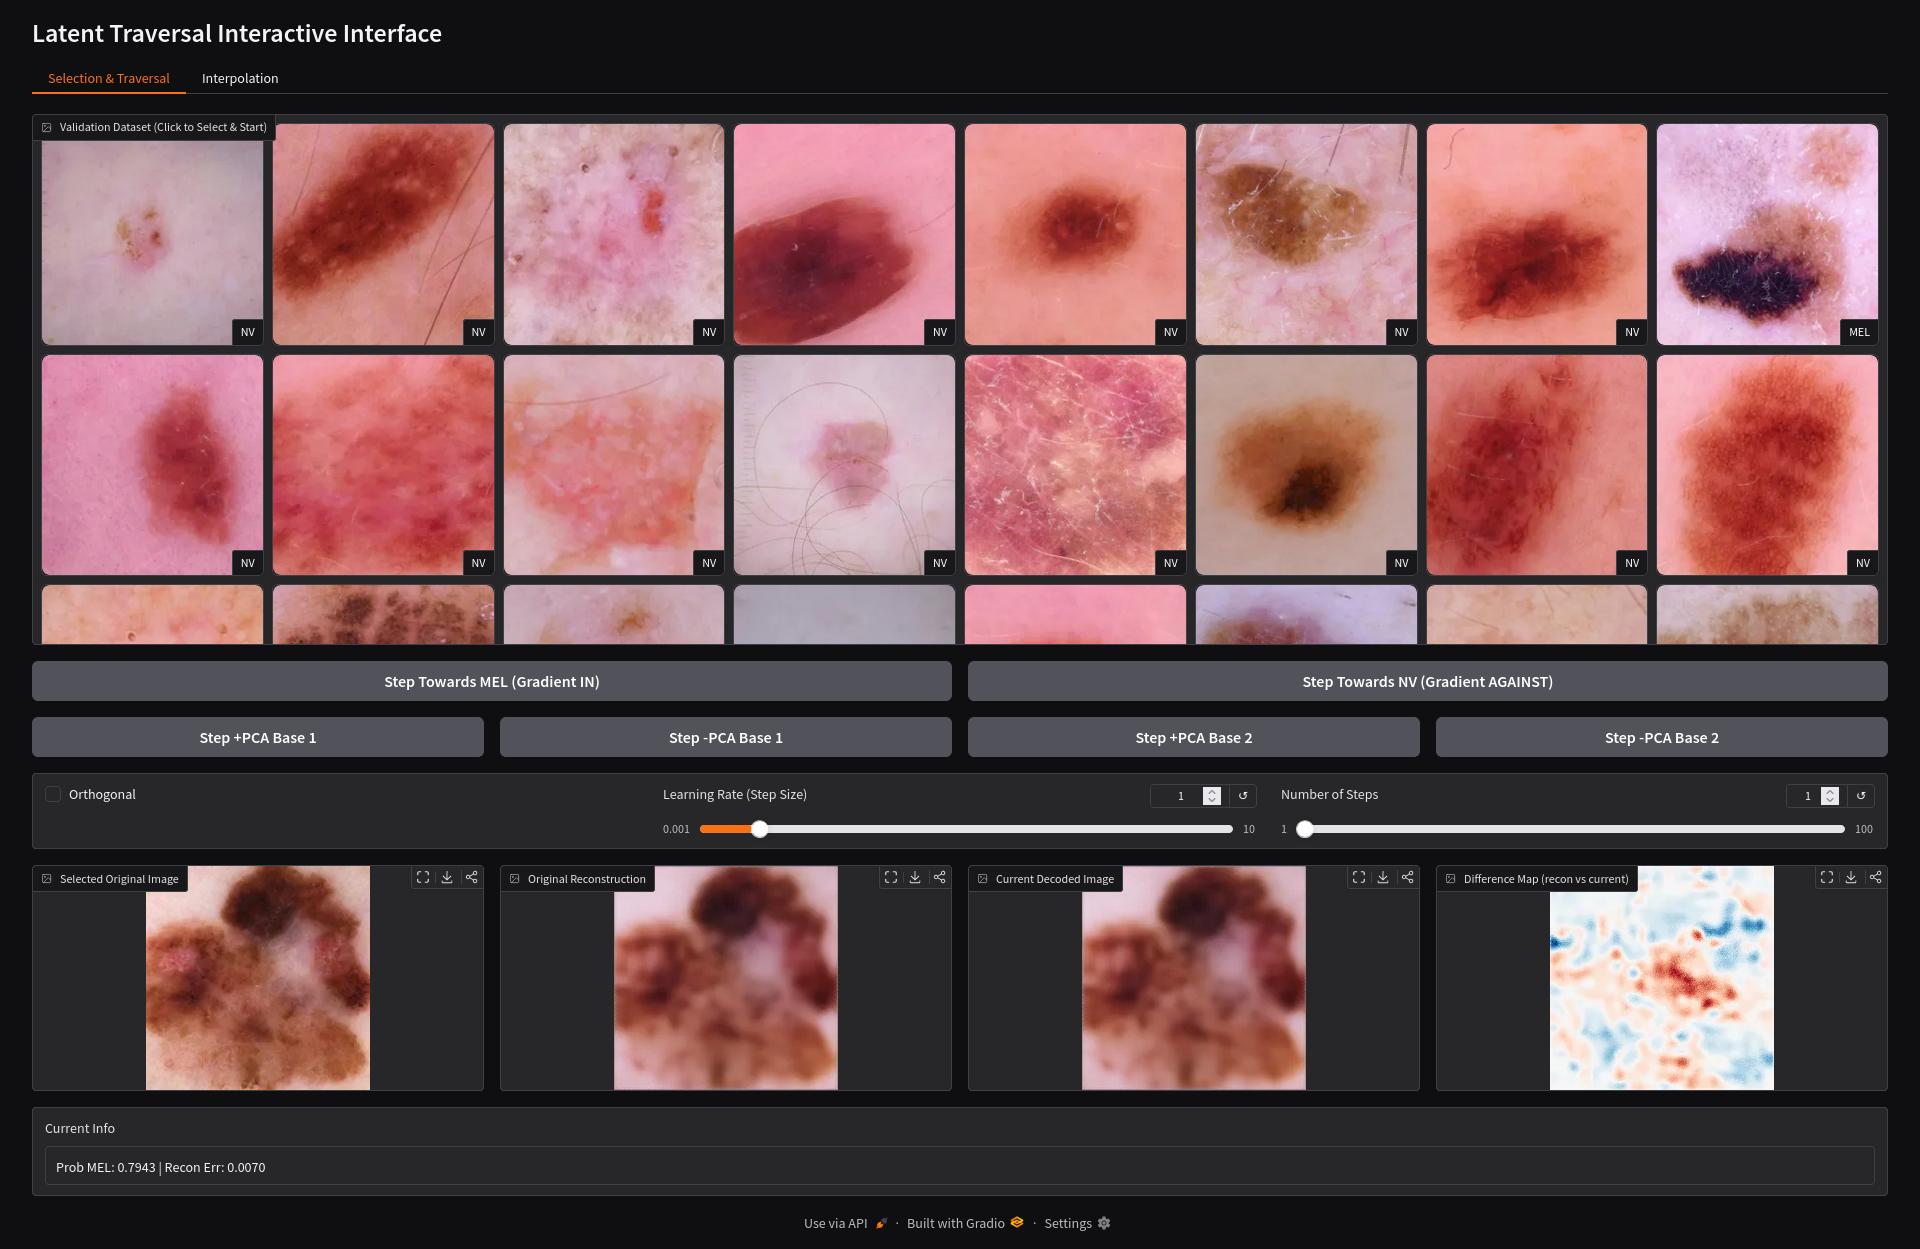
\includegraphics[width=\columnwidth]{images/gui-trav.png}
\caption{The Gradio-based interactive traversal interface. Users select an image and control traversal direction, step size, and the orthogonal constraint in real time.}
\label{fig:gui-trav}
\end{figure}

\begin{figure}[!t]
\centering
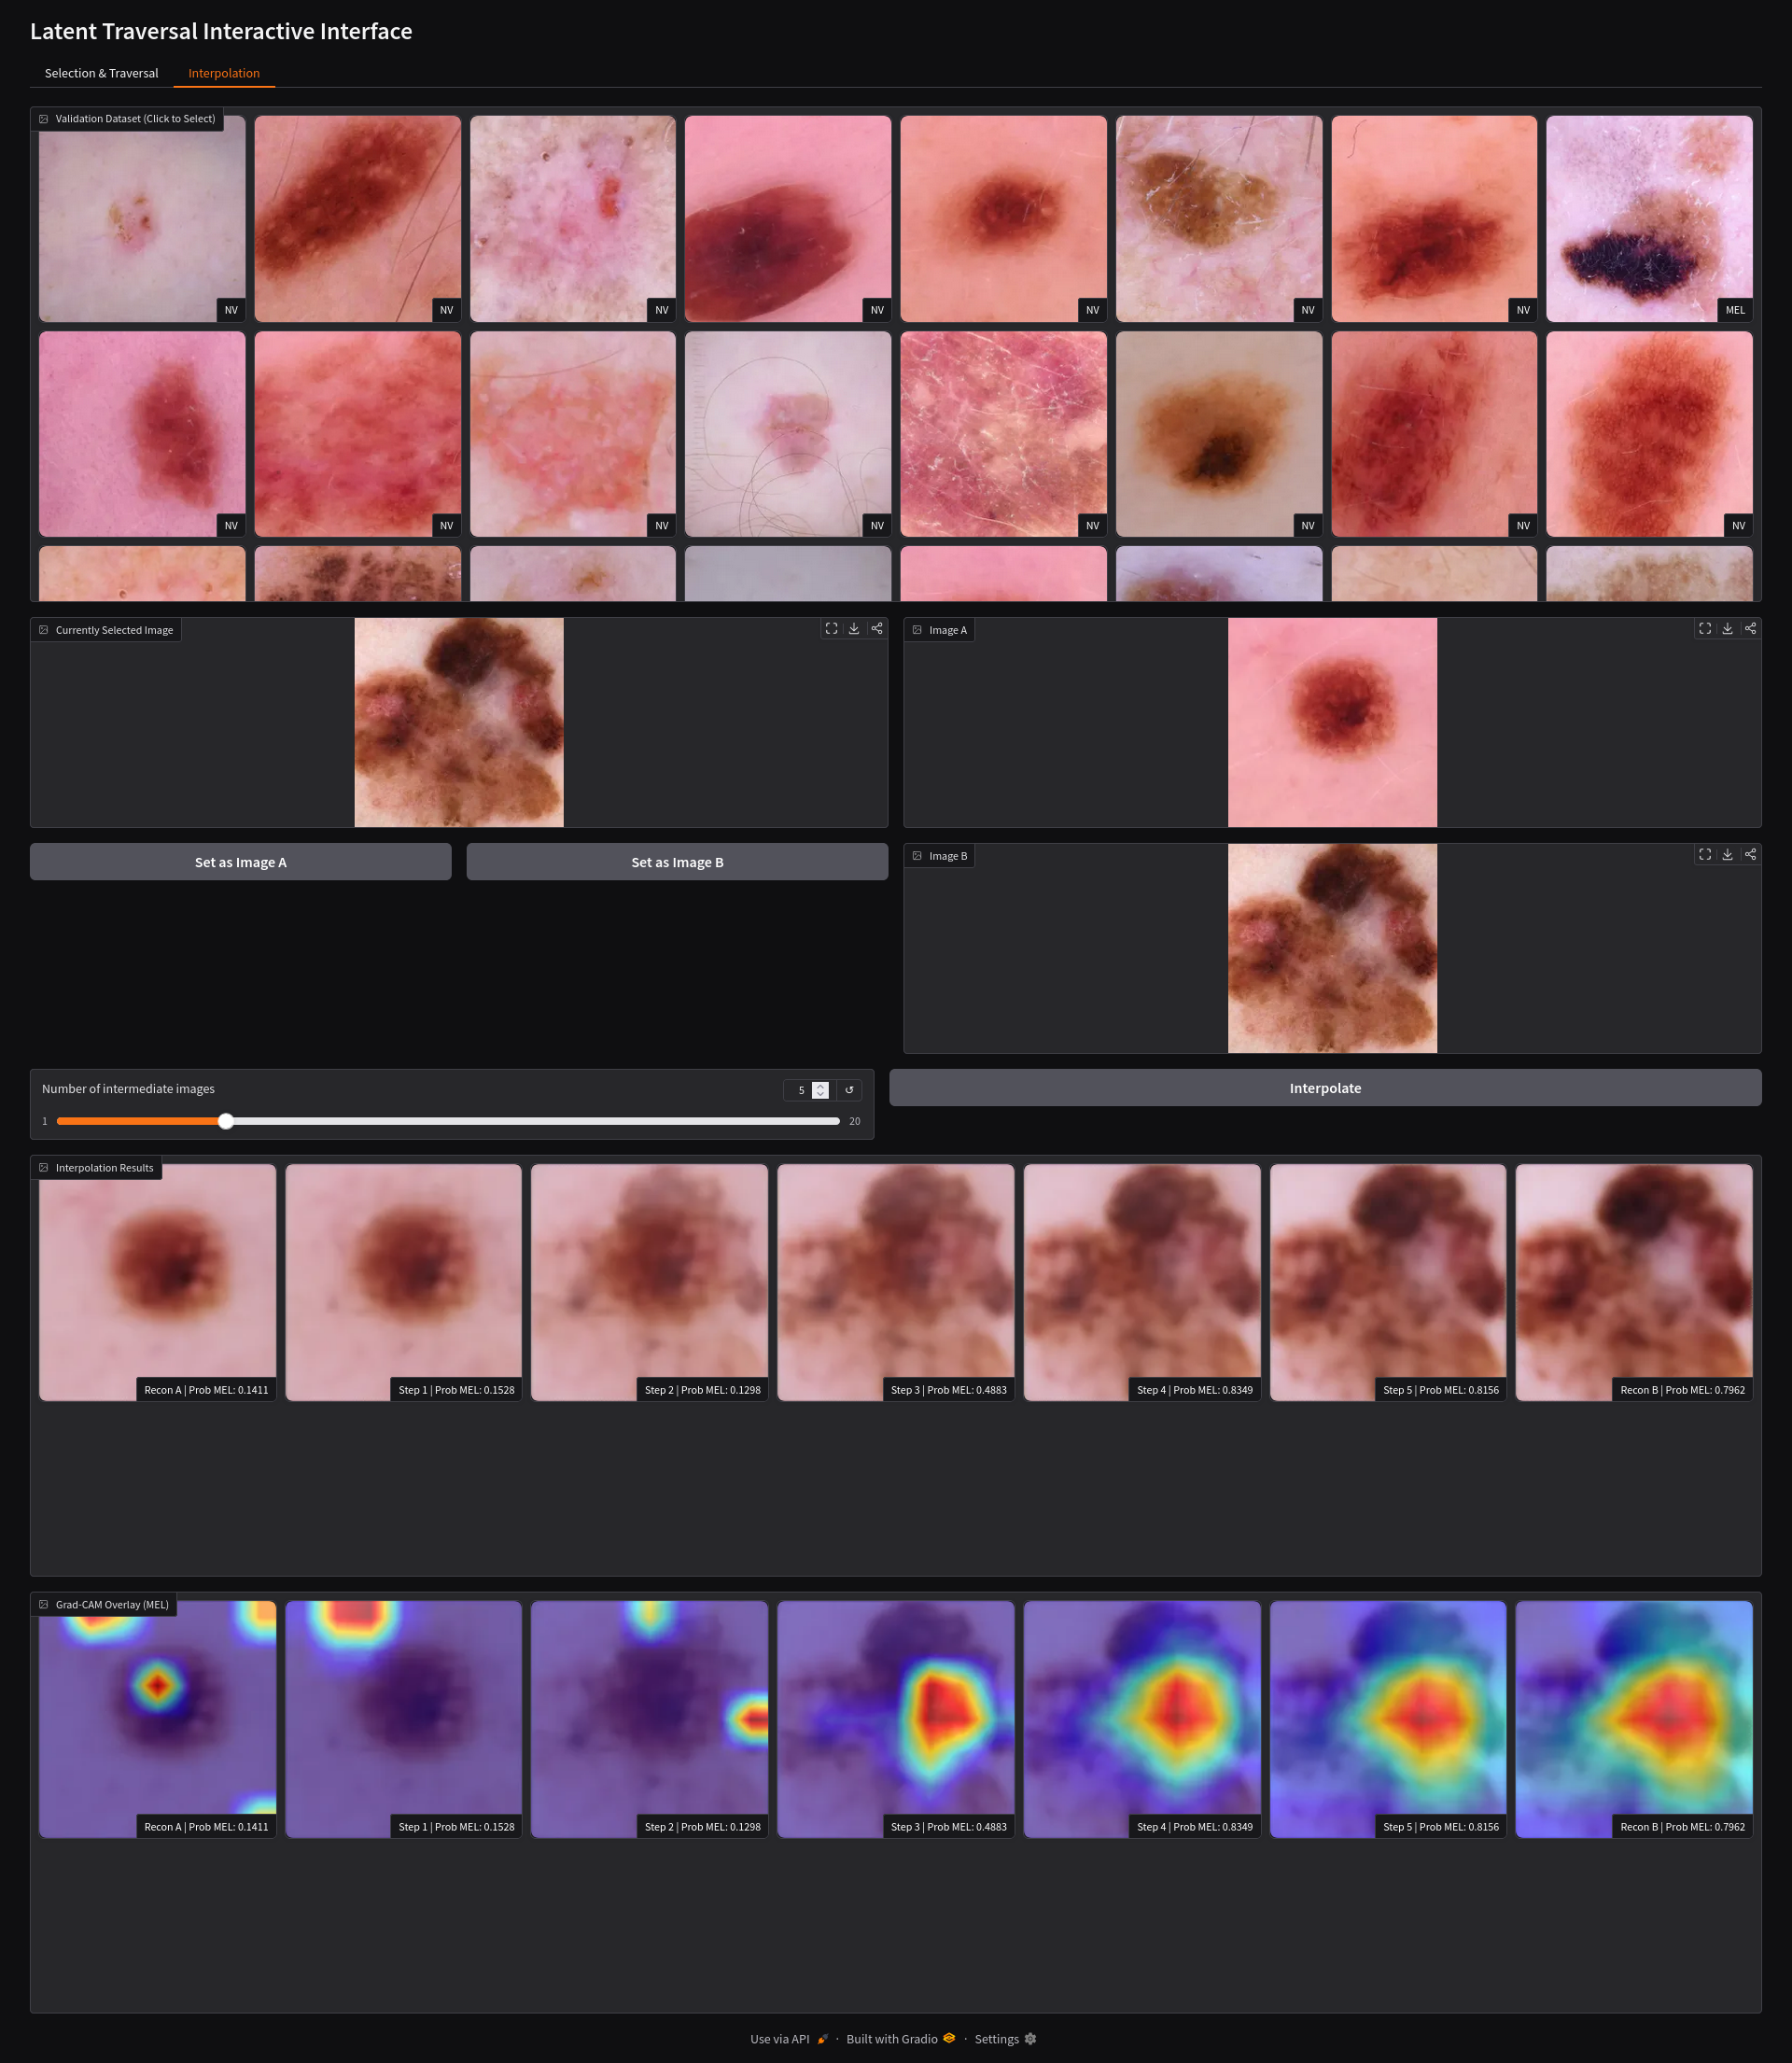
\includegraphics[width=\columnwidth]{images/gui-interpol.png}
\caption{The interpolation view of the GUI. Grad-CAM overlays show which regions drive the classifier's prediction at each point along the interpolation path.}
\label{fig:gui-interpol}
\end{figure}

The interactive web interface is built with Gradio (Fig.~\ref{fig:gui-trav}). It provides three main modes: gradient traversal, PCA traversal, and latent interpolation. In gradient traversal mode, the tool encodes a validation image and takes configurable gradient steps toward the decision boundary, annotating each step with classifier probability, reconstruction error, and gradient norm. In PCA mode, it moves along top PCA bases orthogonal to the classifier gradient, holding confidence score constant while varying visual attributes. In interpolation mode, it linearly interpolates between two latent codes with Grad-CAM attention overlays. All modes update in real time with toggleable orthogonal constraints.

\section{Results}

The orthogonal projection described in Section~\ref{sec:orthogonal} keeps traversal images on the learned manifold, but it comes at a cost: the constraint suppresses visible change so strongly that the latent traversal image is hard to distinguish from the original's reconstruction by eye. This is the price paid to avoid the colour artifacts shown in Fig.~\ref{fig:artifacts}. Whether this trade-off is acceptable depends on how much the orthogonal component can be culled without re-introducing artifacts; future work may explore projecting away only a fraction of the reconstruction-loss gradient rather than removing it entirely.
A more promising signal comes from the gamma-scaled difference map between the latent traversal image and the original's reconstruction. Although the raw decoded frames look nearly identical, the amplified per-channel differences correlate spatially with the Grad-CAM activation of the classifier in some cases but not others, as shown in Fig.~\ref{fig:gamma-diff-gradcam}. Where the two maps agree, it suggests the traversal step moves the latent code in a direction the classifier responds to, even when the decoded change is too subtle for the naked eye; where they disagree, the reasons are discussed below.
\begin{figure}[!t]
\centering
\begin{minipage}[t]{0.48\columnwidth}
    \centering
    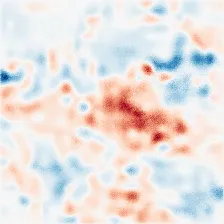
\includegraphics[width=\linewidth]{images/gamma-diff-good.png}
\end{minipage}
\hfill
\begin{minipage}[t]{0.48\columnwidth}
    \centering
    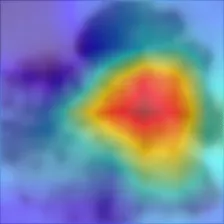
\includegraphics[width=\linewidth]{images/gradcam-good.png}
\end{minipage}
\\[6pt]
\begin{minipage}[t]{0.48\columnwidth}
    \centering
    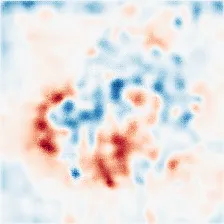
\includegraphics[width=\linewidth]{images/gamma-diff-poor.png}
\end{minipage}
\hfill
\begin{minipage}[t]{0.48\columnwidth}
    \centering
    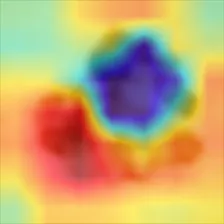
\includegraphics[width=\linewidth]{images/gradcam-poor.png}
\end{minipage}
\caption{Gamma-scaled difference maps (left of each pair) against Grad-CAM activations (right of each pair), for two validation images. Top row: a case where the two maps highlight the same lesion region. Bottom row: a case where they diverge, illustrating that the correlation does not hold consistently.}
\label{fig:gamma-diff-gradcam}
\end{figure}
This correspondence between the difference map and Grad-CAM is the main empirical finding of this paper, but the correlation is not strong, and two factors likely explain why. First, the two maps are built from different signals: Grad-CAM pools gradients over a deep convolutional layer to weight its activation maps, which smooths out much of the noise that raw pixel-space gradients carry, while the gamma-scaled difference map is computed directly in pixel space and has no such smoothing. Some mismatch between the two is expected simply because they are reading the model at different depths. Second, Section~\ref{sec:reconstruction-refinements} shows the classifier does not yet perform as well on reconstructed images as it does on originals; on a poorly reconstructed image, Grad-CAM and the difference map may each be picking up on different decoder noise artifacts rather than the same lesion feature, which would explain why some samples show weaker overlap than others. Fig.~\ref{fig:gamma-diff-gradcam} shows one case of each, annotated accordingly.

This points to what the method actually delivers. The boundary image is the nearest point at which the classifier itself changes its answer, found and verified inside the classifier's own decision space. It is not yet shown to be the nearest point a clinician would recognise as a different case by eye; that would need the decoded image to change visibly, which the orthogonal constraint currently suppresses. The traversal images are not visually compelling on their own, and by that measure the result is weak. But the method's underlying logic holds: gradient steps in latent space do shift classifier-relevant features, and the difference map makes those shifts visible where the decoder cannot. This is enough to warrant further exploration of the approach, particularly with stronger decoders, partial orthogonal projection, and a larger dataset.

\section{Limitations}
Three questions remain open and would need more work than this paper covers. First, boundary-image plausibility was not measured quantitatively; a distributional check such as the Fr\'echet Inception Distance (FID), which compares the feature statistics of two image sets to score how close a generated set is to a set of real images \cite{fid}, would show whether decoded boundaries stay close to the true image manifold rather than only avoiding the colour artifacts of Fig.~\ref{fig:artifacts}. Second, no clinician has reviewed the boundary or traversal images; the tool is described as clinician-facing by design, not by evaluation. Third, Fig.~\ref{fig:gamma-diff-gradcam} shows the difference-map/Grad-CAM correspondence holds for one example and not another; a quantitative overlap metric such as IoU or cosine similarity, measured across the full validation set, would give a clearer picture of how often it holds, though such a metric would inherit the same limitation discussed above: it would still be comparing a pixel-space map against a deep-layer activation map, on reconstructions the classifier has not yet mastered, so a low score would not on its own separate a true mismatch from an artefact of the metric itself.

\section{Conclusion}
We built a tool that encodes skin lesion images into a latent space and traverses it to expose a binary classifier's decision boundary. The core output is a boundary image at the point where the classifier flips label. As it stands, this boundary is defined and verified in the classifier's own decision space; it is not yet shown to be a boundary a clinician would recognise as visually distinct, since the current decoder keeps changes small enough that the difference map, not the raw image, carries most of the signal. Closing that gap is the paper's main open problem. MS-SSIM reconstruction loss, orthogonal gradient projection, and fine-tuning on reconstructions together produce a usable system. The Gradio interface makes the latent space interactive without requiring any machine learning knowledge from the clinician.

Several directions remain for future work. First, combining VGG perceptual loss with MS-SSIM offers a path toward sharper reconstructions, alongside extending the pipeline to multiclass settings. Second, deploying a GAN-style decoder could yield more realistic textures and raise classifier fidelity on reconstructed inputs, thereby strengthening the correlation between difference maps and Grad-CAM activations. However, given our limited dataset size ($\sim 1{,}100$ melanoma images), adversarial training carries stability risks such as mode collapse, making non-adversarial alternatives like diffusion autoencoders \cite{daecf} a promising alternative. Finally, addressing key limitations (evaluating boundary image plausibility via FID, conducting clinician user studies, and measuring spatial overlap metrics across the validation set) will be essential to fully establish clinical utility.

\bibliographystyle{IEEEtran}
\bibliography{references}

\end{document}